\section{Exploratory analyses of norm weighting}\label{app:explore}
\paragraph{Deletion endpoints.} For each image and method, trapezoidal integration uses the original removal budgets, divided by 196. The probability endpoint integrates the probability of the original top-1 class under least-important-first removal minus most-important-first removal. The KL endpoint uses the reverse difference in divergence from the original prediction, so that larger scores again indicate greater separation. For both endpoints the paired curve difference is zero at budget zero. Results are paired over images. These measures have no registered practical margin.
\paragraph{Uncertainty.} Differences are paired by image. Intervals use 1,000 image-bootstrap resamples with seed 0. ClickMe reuses each human map within a batch for its own and another image. Recomputing intervals by sampling the 272 original 64-image batches preserves those dependencies. For C3 relative to zeroing high-norm patches, the resulting ClickMe intervals are [0.021, 0.023] in DeiT-S and [0.016, 0.018] in DeiT-B. All estimates condition on the fixed within-batch pairing and the available checkpoints.
\begin{center}\begin{minipage}{\linewidth}
\captionof{table}{Exploratory endpoint differences (C3 minus comparator). Probability and KL columns give the mean paired area and 95\% image-bootstrap interval over the fixed 2,000-image deletion subset. ClickMe uses the original 17,408 images with batch-bootstrap intervals. KL has units of nats times fraction removed.}
\centering\footnotesize\setlength{\tabcolsep}{3pt}
\begin{tabular}{@{}llrrr@{}}
\toprule
Model & Comparator & Probability area & KL area & ClickMe \\
\midrule
DeiT-S & R0 & 0.014 [0.012, 0.015] & 0.058 [0.050, 0.066] & 0.033 [0.032, 0.034] \\
DeiT-S & Zero high-norm & 0.010 [0.009, 0.012] & 0.041 [0.033, 0.049] & 0.022 [0.021, 0.023] \\
DeiT-B & R0 & 0.022 [0.020, 0.024] & 0.107 [0.096, 0.118] & 0.058 [0.056, 0.059] \\
DeiT-B & Zero high-norm & 0.010 [0.008, 0.012] & 0.048 [0.038, 0.058] & 0.017 [0.016, 0.018] \\
DINO & R0 & 0.000 [$-$0.001, 0.002] & $-$0.003 [$-$0.009, 0.003] & $-$0.001 [$-$0.001, $-$0.001] \\
DINO & Zero high-norm & 0.000 [$-$0.001, 0.002] & $-$0.003 [$-$0.009, 0.003] & $-$0.001 [$-$0.001, $-$0.001] \\
\bottomrule
\end{tabular}

\end{minipage}\end{center}
\begin{center}\begin{minipage}{\linewidth}
\centering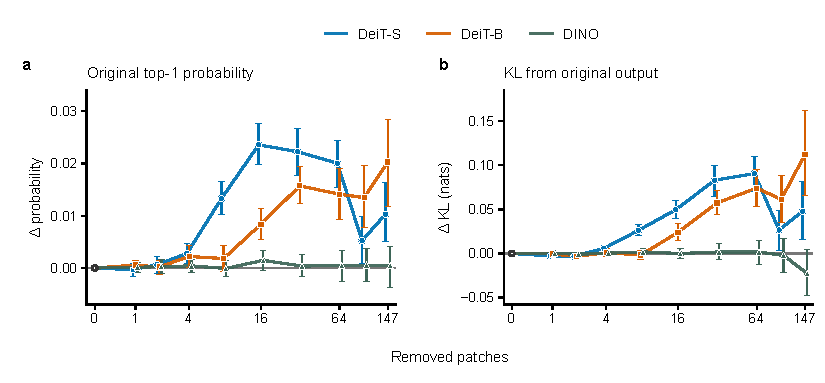
\includegraphics[width=\linewidth]{../../research/v13/endpoints/deletion_curves.pdf}
\captionof{figure}{C3 minus the zero-high-norm control at each original ImageNet-S deletion budget. The probability panel measures least-important-first minus most-important-first target probability. The KL panel reverses the subtraction to express divergence in the same direction. Horizontal positions use a log scale in one plus the number of removed patches, with model-specific offsets for visibility. Intervals are pointwise 95\% paired image-bootstrap intervals over 2,000 images per model. The integrated advantage can coexist with a reversal at a small budget.}
\end{minipage}\end{center}

\clearpage
\subsection{Object geometry and the enrichment scale}
For an image with $M$ valid patches and $k>0$ foreground patches, let ring $r$ contain $m_r$ valid patches of which $f_r$ are foreground. Selecting a patch in this ring contributes $(y-f_r/m_r)/k$ to enrichment, where $y$ is its foreground indicator. Foreground contributions are nonnegative and background contributions are nonpositive. Selecting all $k$ foreground patches therefore attains the maximum
\[
 E_{\max}=1-\frac{1}{k}\sum_{r:m_r>0}\frac{f_r^2}{m_r}\ \le\ 1-\frac{k}{M}.
\]
The inequality follows by Cauchy--Schwarz. It bounds the score itself. The possible change from R0 also depends on R0's starting score. A large raw improvement for small objects can thus reflect properties of both the map and the metric.
\paragraph{Area and centroid displacement.} Object area is the share of valid patch slots labelled foreground. Centroid displacement is the distance from their centroid to the grid centre, in patches. For each checkpoint we computed the empirical quartiles on its finite-geometry images, assigning ties to the lower bin. The DeiT area cut points were 0.158, 0.342 and 0.571. DINO's different crop produced different masks. We paired scores within the same supplementary run and resampled images 2,000 times. In DeiT-S and DeiT-B the largest-minus-smallest area quartile differences in the C3 gain were $-0.090$ and $-0.157$ for enrichment. Comparing the most off-centre with the most central quartile instead gave $+0.057$ and $+0.095$. Area and centroid displacement covary. Among the smallest objects the latter differences were $+0.041$ [0.028, 0.053] and $+0.047$ [0.028, 0.066]. Some joint bins are small and these are observational contrasts.

\paragraph{Metric sensitivity.} After seeing the enrichment gradients we examined patch AUROC under the same quartile cut points. AUROC is the probability that a foreground patch outranks a background patch, counting ties as one half. In the supervised models the gain in AUROC persists across area quartiles (Table~\ref{tab:geometry}). AUROC does not condition on radius, so this comparison changes spatial adjustment as well as how foreground patches are selected. Overall C3-minus-R0 AUROC changes are $+0.028$, $+0.046$ and $-0.005$ for DeiT-S, DeiT-B and DINO.

\paragraph{Historical sample membership.} Archived ImageNet-S files record zero enrichment for all-foreground grids, as the ring formula implies. Counts are 241 such grids for each DeiT and 265 for DINO. An additional 269/275 images, respectively, have zero object area and are excluded from the archived enrichment means. AUROC requires both classes, giving 11,909 DeiT and 11,879 DINO images. Restricting enrichment to that common eligibility changes C3-minus-R0 from 0.03757 to 0.03833 in DeiT-S, 0.06539 to 0.06671 in DeiT-B and $-0.00351$ to $-0.00359$ in DINO. The original verdicts use the archived cohort. In two DeiT-S images the original and supplementary R0 exports differ slightly. The stratified comparisons pair both methods from the supplementary export.

\begin{center}\begin{minipage}{\linewidth}
\captionof{table}{Mean C3 minus R0 by foreground-area quartile on ImageNet-S. Q1 contains the smallest objects. Both metrics use the same within-model cut points. AUROC excludes all-foreground crops.}
\label{tab:geometry}\centering\small\begin{tabular}{@{}llrrrr@{}}
\toprule
Metric & Model & Q1 & Q2 & Q3 & Q4 \\
\midrule
Enrichment & DeiT-S & 0.092 & 0.041 & 0.013 & 0.002 \\
Enrichment & DeiT-B & 0.165 & 0.060 & 0.026 & 0.008 \\
Enrichment & DINO & $-$0.003 & $-$0.004 & $-$0.005 & $-$0.003 \\
AUROC & DeiT-S & 0.024 & 0.030 & 0.031 & 0.026 \\
AUROC & DeiT-B & 0.042 & 0.048 & 0.048 & 0.046 \\
AUROC & DINO & 0.000 & $-$0.002 & $-$0.006 & $-$0.013 \\
\bottomrule
\end{tabular}

\end{minipage}\end{center}

\clearpage
\subsection{Independent pet-image controls}
The Oxford release provides test filenames and trimaps. We sorted filenames by SHA-256 of the fixed prefix and name (protocol under \texttt{research/v13/spatial/}), taking the first 384. Images were resized on the short side to 248 pixels with bicubic interpolation and centre-cropped to 224. The masks received the same spatial transform with nearest-neighbour interpolation. Label 3 (boundary) was ignored. A patch counted as foreground when at least half its valid pixels were foreground. One crop contained only foreground. Each image and its adjacent partner in hash order exchanged norm rankings. In each within-ring shuffle all heads shared a permutation for that image and layer. The recipient's sorted values, head scales and marginal distributions were preserved by rank transfer. Norm-only sets each head's received attention to its spatial mean before multiplying by its patch-specific length.

All seven readouts were evaluated on identical masks. Primary intervals used 10,000 paired image-bootstrap draws (seed 2026). A follow-up sensitivity check resampled the 192 donor pairs, weighting by the number of eligible images in each draw. C3 minus donor-rank gives 0.0223 [0.0187, 0.0261] in this check. The captured C3 map and logits were checked against the original implementation on the first batch. Each query--patch pair satisfied the triangle bound within numerical tolerance over the run. Public Oxford images and the model weights are available from their original providers. Individual scores, selected IDs, scripts and protocols accompany the source.
\subsection{Last-block CLS value intervention}
A second fixed filename hash selected 128 of the 384 images independently of their scores. At block 12 we cached its input and the unmodified logits. For each patch $j$ we held the original CLS attention weights fixed and removed $t_j=\sum_h a^h_{\mathrm{CLS},j}z_j^h$ from the CLS attention output. The shared projection bias stayed in place. The remaining residual, token-wise MLP, final normalisation and classifier were evaluated for each modified CLS. If $m$ is the margin between the original highest and second-highest logits, the response was $|m_{-j}-m|$ for those same classes. This intervention concerns the contextualised token at that slot. Its input evidence can span multiple image regions.

For each image, we correlated the 196 responses with each unmodified layer-12 readout by Spearman correlation. The means over images were 0.696 (all-query R0), 0.705 (all-query C3), 0.730 (CLS attention), 0.747 (CLS sum of head magnitudes) and 0.756 (CLS net magnitude). The paired CLS-only sum versus all-query C3 difference was 0.041 [0.026, 0.057] with 10,000 image-bootstrap resamples. Explicit interventions in full forward passes on four images and three patch indices each agreed with vectorised logits to within $2.4\times10^{-6}$. The 128-image run took about 3 seconds on the RTX 4060 with inputs cached. The supplied scripts and individual patch responses are under \texttt{research/v13/cls/}.
\paragraph{Matched mask comparison.} After inspecting the classifier intervention we evaluated the saved layer-12 rankings on the same 128 images and masks. All 128 had eligible foreground and background patches. Table~\ref{tab:cls} reports the three outcomes with equal image weights. Keeping the CLS query fixed, moving from the sum of per-head magnitudes to net magnitude changed margin Spearman by $+0.0092$ [0.0069, 0.0116], enrichment by $+0.0037$ [0.0007, 0.0069] and AUROC by $+0.0002$ [$-0.0031$, 0.0033]. The target margin uses the direct path queried by the CLS-specific score. These observations describe that layer and intervention. They do not identify the pixels responsible for earlier token representations.


